\documentclass[11pt]{article}
\usepackage[letterpaper,margin=0.9in]{geometry}
\usepackage{graphicx,booktabs,longtable,tabularx,array,enumitem,xcolor,fancyhdr}
\usepackage{xurl,tikz,caption}
\captionsetup{font=small}
\usepackage[hidelinks]{hyperref}
\usepackage{helvet}\renewcommand{\familydefault}{\sfdefault}
\definecolor{accent}{HTML}{1F4E79}
\setlist{itemsep=2pt,topsep=3pt}
\pagestyle{fancy}\fancyhf{}\lhead{\small RC Mini Cat 600: Build Manual}\rhead{\small F. Maleev}\cfoot{\small\thepage}
\newcommand{\step}[1]{\subsection*{\color{accent}#1}}
\newcommand{\chk}[1]{\par\noindent\textbf{Check:} #1\par}
\begin{document}
\begin{titlepage}
\centering
{\Huge\bfseries RC Mini Cat 600\par}\vspace{4pt}
{\Large Build Manual and Costed Parts List\par}\vspace{6pt}
{\large A simplified 600\,mm version of the RC Foiling Catamaran project\par}\vspace{14pt}
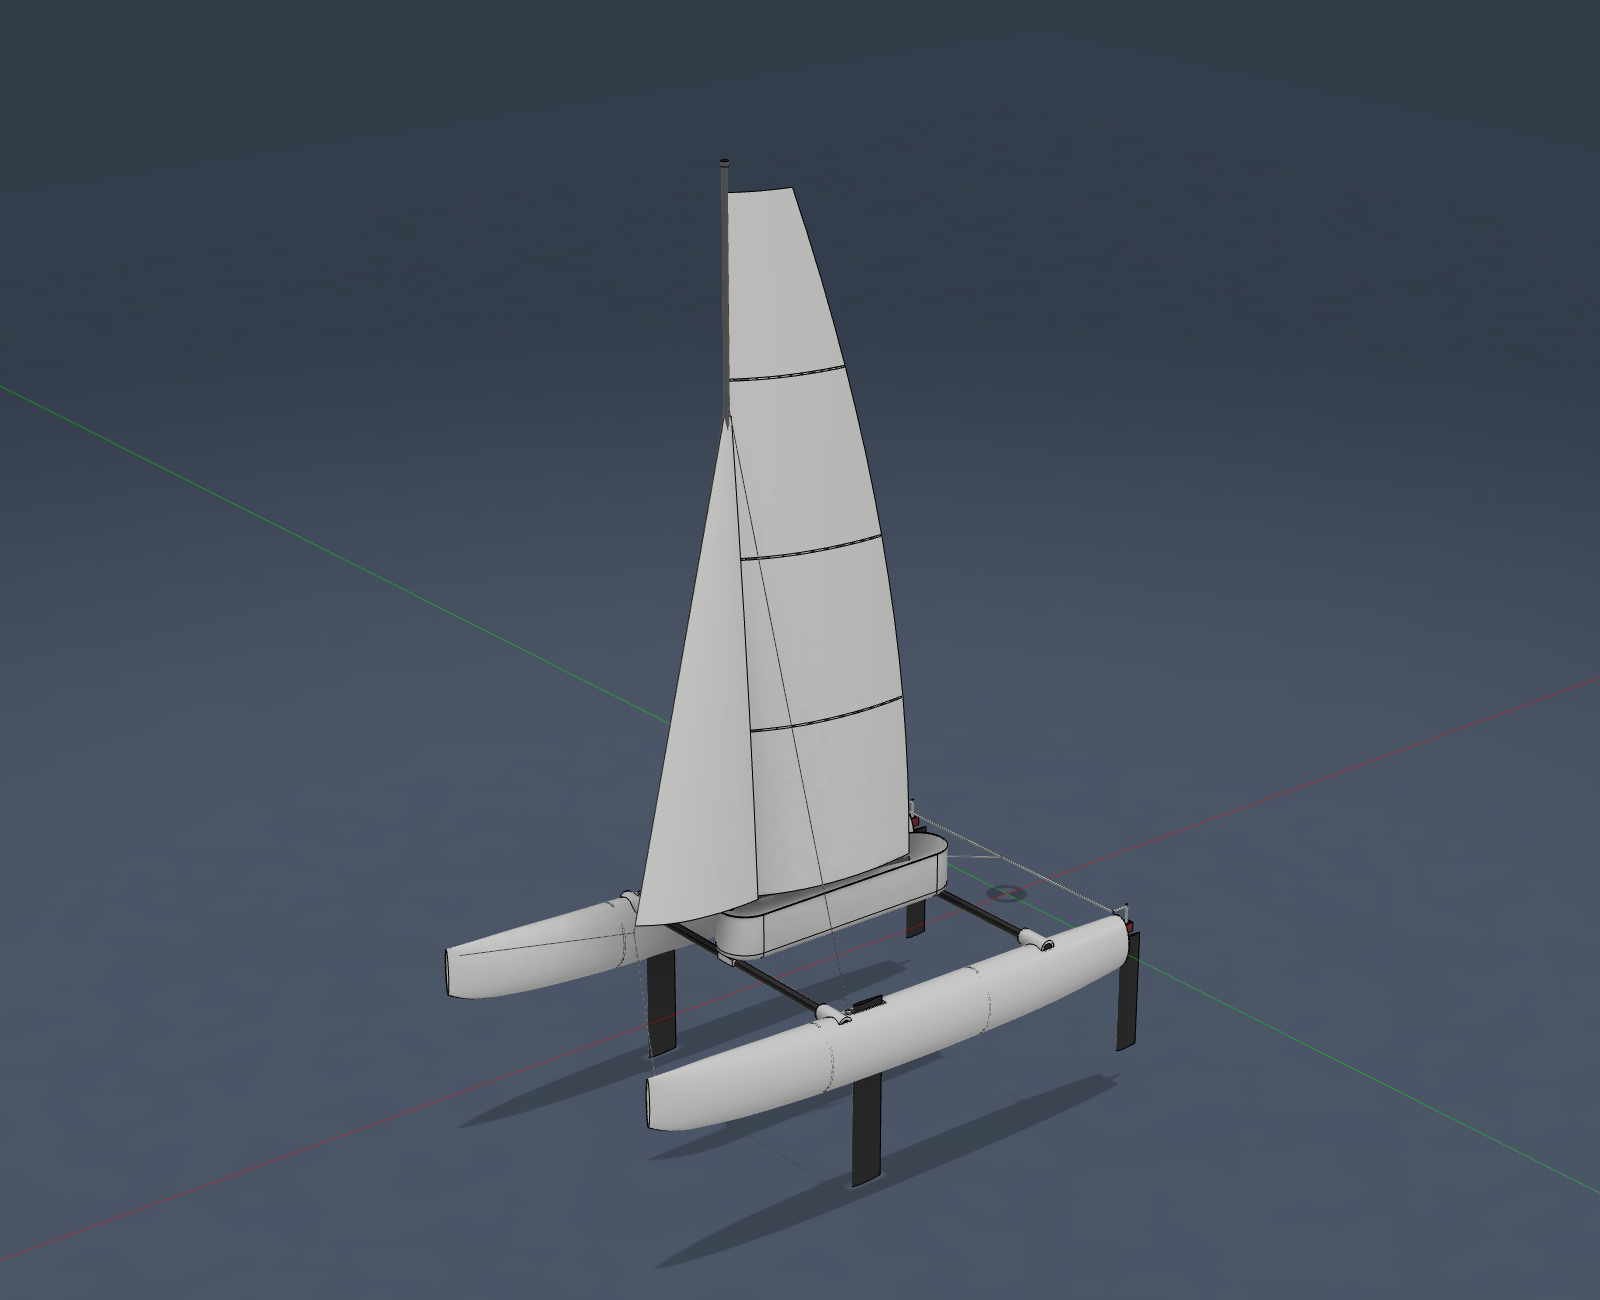
\includegraphics[width=0.78\textwidth]{../images/mini_iso.png}\par\vspace{10pt}
\begin{tabular}{ll}
\toprule
Length / overall beam & 600 mm / 394 mm \\
Sailing mass (estimate) & 755 g \\
Sail area (main + jib) & 0.143 m$^2$ \\
Radio & 2 channels used: rudder + one sail winch \\
Parts cost (USD, Sep 2026) & \textbf{\$248.26} \\
\bottomrule
\end{tabular}\par\vfill
{\large Filip Maleev\par September 2026\par}
\end{titlepage}

\section{What you are building}
The Mini Cat is the smallest step toward the 1\,m RC catamaran: the same hull lines (scaled 0.6 in length and 0.68 in section), the same beach-cat sail plan (square-top main with 3 full-length battens, jib on a forestay bridle), and the same printed-hull construction (0.8\,mm PETG skin, every print segment a sealed compartment). It keeps what matters for learning to build and sail the big boat and drops what makes the big boat hard.

\begin{center}
\begin{tabularx}{\textwidth}{>{\raggedright}p{3.3cm}XX}
\toprule
& \textbf{1\,m boat (build-first v1.2)} & \textbf{Mini Cat 600 (this manual)} \\
\midrule
Sail controls & 3 servos: jib sheet, traveler, mainsheet tension & 1 winch pulls both sheets on a stepped drum \\
Mast & rotating wing mast & fixed 6\,mm carbon tube \\
Main battens & 8 & 3 \\
Mainsheet & traveler car on the rear beam & fixed fairlead on the box lid \\
Hull pieces to print & 10 (5 per hull) & 6 (3 per hull) \\
Radio channels used & 4 & 2 \\
Parts cost & \$397.74 & \$248.26 \\
\bottomrule
\end{tabularx}
\end{center}

\subsection*{Predicted numbers (from the project's analysis code; not yet measured on the water)}
\begin{itemize}
\item Floats with the hulls 24\,mm deep and 50\,mm of freeboard at mid-length; level trim (centre of buoyancy 262\,mm, centre of gravity 258\,mm from the transom).
\item Each hull alone could float 2.05 times the boat's weight (design target 2 or more).
\item Speed on a beam reach: 0.95\,m/s in 4\,kn of wind, 2.13\,m/s in 8\,kn. The rig must be eased (depowered) above about 8\,kn close-reaching and 11\,kn on a beam reach.
\item Steering: at most 1.6$^\circ$ of rudder is needed of the 19.9$^\circ$ the linkage gives, leaving at least 86\,\% margin before the rudders stall.
\end{itemize}

\section{What it costs}
\begin{center}
\begin{tabular}{lr}
\toprule
\textbf{Group} & \textbf{Cost} \\
\midrule
Radio & \$72.98 \\
Servos & \$13.72 \\
Power & \$21.99 \\
Printed & \$13.99 \\
Carbon & \$43.36 \\
Hardware & \$20.52 \\
Sails & \$28.49 \\
Rigging & \$14.43 \\
Adhesives & \$18.78 \\
\midrule
\textbf{Total parts} & \textbf{\$248.26} \\
\bottomrule
\end{tabular}
\end{center}
Prices were read on the retailers' pages on 23 September 2026 and re-checked on 4 October 2026 (links in Appendix C). Not included: shipping (HobbyTown charges a \$3.99 flat rate; other stores vary), sales tax, a NiMH charger for the eneloop cells, the 3D printer, paint, and hand tools. The FS-i6X radio is the largest single item and is reused unchanged for the 1\,m boat.

\noindent\textbf{Choices.} Where a part has a cheaper or better option, the list uses the recommended one. The alternatives, with the pros and cons of each:
{\small
\begin{longtable}{p{3.6cm}rp{5.2cm}p{5.2cm}}
\toprule
Option & Unit & Pros & Cons \\
\midrule\endhead
Listed: FlySky FS-i6X + FS-iA6B receiver & \$69.99 & 6 channels, so one radio runs both boats; the throttle stick stays where you leave it, which holds a sail trim & \$31 more than the car radio \\
Cheaper, Mini only: FlySky FS-GT2E + FS-A3 (car radio) & \$38.99 & \$31 less & 2 channels, so it cannot run the 1 m boat (you would buy the FS-i6X later as well); the throttle trigger springs back to centre, so a sail trim has to be held by hand \\
\midrule
Listed: MG90S metal-gear micro servo & \$2.59 & \$2.59; the printed servo rails are drawn to its case & not waterproof; on the 1 m boat it sits under a printed cover aft of the rear beam, where spray reaches \\
Upgrade: EcoPower 640T waterproof micro servo & \$29.99 & waterproof to 1 m and metal-geared (maker); rated 4.8-6.0 V, so it runs on the 4.8 V pack & \$27.40 more; its case is 23.5 x 12.5 mm against the MG90S 22.8 x 12.2 mm, so it does not fit between the printed rails (23.4 mm gap) unless they are widened \\
\midrule
Listed: Panasonic eneloop AA 2000 mAh, 4-pack & \$17.99 & in stock when checked (2026-10-04) & \$5.24 more; sold by a third-party seller on Walmart \\
Cheaper: The same eneloop 4-pack at MicroBattery & \$12.75 & \$5.24 less & out of stock when checked (2026-10-04) \\
\midrule
Listed: BSI 30-minute epoxy 4.5 oz & \$13.99 & the strongest of the BSI epoxies, waterproof and more heat resistant (maker); 30 minutes to line up hull segments and beams before it sets & handle after 8 hours, full strength in 24 hours (maker) \\
Same price, faster: BSI 5-minute epoxy 4.5 oz & \$13.99 & sets in minutes: handy for small fittings & weaker, and 5 minutes is short for lining up a long hull or beam joint \\
\bottomrule
\end{longtable}}

\section{Parts list}
{\small
\begin{longtable}{p{1.5cm}p{4.3cm}p{5.0cm}cp{1.2cm}p{1.2cm}}
\toprule
\textbf{Group} & \textbf{Item} & \textbf{Used for} & \textbf{Qty} & \textbf{Unit} & \textbf{Total} \\
\midrule\endhead
Radio & FlySky FS-i6X + FS-iA6B receiver & CH1 rudder, CH3 sails (non-centering stick); reused on the 1 m boat & 1 & \$69.99 & \$69.99 \\
Radio & AA alkaline x4 & transmitter power & 1 & \$2.99 & \$2.99 \\
Servos & JX W4505-2T sail winch servo & both sheets on the stepped drum & 1 & \$11.13 & \$11.13 \\
Servos & MG90S metal-gear micro servo & rudders via pushrod + tie bar & 1 & \$2.59 & \$2.59 \\
Power & Panasonic eneloop AA 2000 mAh, 4-pack & receiver pack (4.8 V) & 1 & \$17.99 & \$17.99 \\
Power & Traxxas 4-cell AA holder with switch (TRA1523) & receiver battery box + on/off & 1 & \$4.00 & \$4.00 \\
Printed & PETG filament 1 kg & hulls, box, lid, rudders, boards, drum (~470 g used) & 1 & \$13.99 & \$13.99 \\
Carbon & Carbon tube 10 x 8 mm x 1 m & two 360 mm crossbeams & 1 & \$16.15 & \$16.15 \\
Carbon & Carbon tube 6 x 4 mm x 1 m & mast (800 mm) & 1 & \$15.25 & \$15.25 \\
Carbon & Carbon tube 4 mm OD x 1 m & boom (210 mm) & 1 & \$8.49 & \$8.49 \\
Carbon & Carbon rod 1.2 mm x 1 m & 3 battens & 1 & \$3.47 & \$3.47 \\
Hardware & Music wire 0.125 in & rudder stocks & 1 & \$3.99 & \$3.99 \\
Hardware & Music wire 0.093 in & tie bar, tiller arms & 1 & \$3.99 & \$3.99 \\
Hardware & Music wire 0.047 in & rudder pushrod, sheet hooks & 1 & \$3.99 & \$3.99 \\
Hardware & Du-Bro micro pushrod system & clevis + tube for the rudder pushrod & 1 & \$8.55 & \$8.55 \\
Sails & Icarex PC31 ripstop polyester, 1 m & main + jib (0.145 m2) & 1 & \$21.99 & \$21.99 \\
Sails & Ripstop sail tape 2 in, 10 ft & luff, batten pockets, corners & 1 & \$6.50 & \$6.50 \\
Rigging & Braided PE line 30 lb & stays, bridle, sheets & 1 & \$14.43 & \$14.43 \\
Adhesives & BSI 30-minute epoxy 4.5 oz & hull segment joints, beams, fittings & 1 & \$13.99 & \$13.99 \\
Adhesives & BSI gap-filling CA 1/2 oz & small parts, knots & 1 & \$4.79 & \$4.79 \\
\midrule
& \textbf{Total} & & & & \textbf{\$248.26} \\
\bottomrule
\end{longtable}}

\subsection*{Tools and shop supplies (assumed on hand)}
3D printer with a 220\,mm bed that prints PETG; hobby knife and a steel rule; drill bits 1.2, 1.5, 2.5 and 3.2\,mm (a pin vise is enough); side cutters and round-nose pliers for bending music wire; 240-grit sandpaper; masking tape; a fine-tip soldering iron or a hot needle to melt clean holes in the sailcloth; small screwdrivers for servo screws; a bucket or sink for leak tests; a kitchen scale.

\section{Printing}
Settings used for the design mass: PETG, 0.4\,mm nozzle, 0.2\,mm layers, \textbf{2 perimeters (0.8\,mm walls)} for hulls, box and lid, 5 top and 5 bottom layers, \textbf{0\,\% infill} for the hull segments (they are closed shells: each segment prints as a sealed compartment ending in half of a 2\,mm bulkhead). Rudders, daggerboards and the drum are solid parts: 3 perimeters and 40\,\% infill. About 462\,g of the 1\,kg spool is used.
\begin{center}
{\small
\begin{tabular}{lllll}
\toprule
\textbf{Part} & \textbf{Qty} & \textbf{g each} & \textbf{Size (mm)} & \textbf{Orientation / notes} \\
\midrule
Hull Port Seg 1 / 2 / 3 & 1 each & 44 / 56 / 38 & 200 x 55 x 78 & stand on the joint (bulkhead) face \\
Hull Stbd Seg 1 / 2 / 3 & 1 each & 44 / 56 / 38 & 200 x 55 x 78 & mirror of port \\
Box Half 1 / 2 & 1 each & 37 / 42 & 144 x 60 x 56 & open side up \\
Box Lid Half 1 / 2 & 1 each & 10 / 10 & 144 x 60 x 1 & flat \\
Daggerboard & 2 & 27 & 200 x 36 x 4.3 & flat; 3 perimeters, 40 \% infill \\
Rudder Blade & 2 & 10 & 130 x 27 x 3.2 & flat; 3 perimeters, 40 \% infill \\
Gudgeon & 2 & 2 & 18 x 10 x 10 & any \\
Winch Drum (30 / 16.2 mm) & 1 & 7 & 34 x 34 x 10.4 & large flange down \\
\bottomrule
\end{tabular}}
\end{center}
Files: \texttt{mini/stl/} (STL, one file per part), \texttt{mini/cad/RC\_Mini\_Cat\_600.step} and \texttt{.f3d} (full assembly).

\section{Build steps}
\begin{center}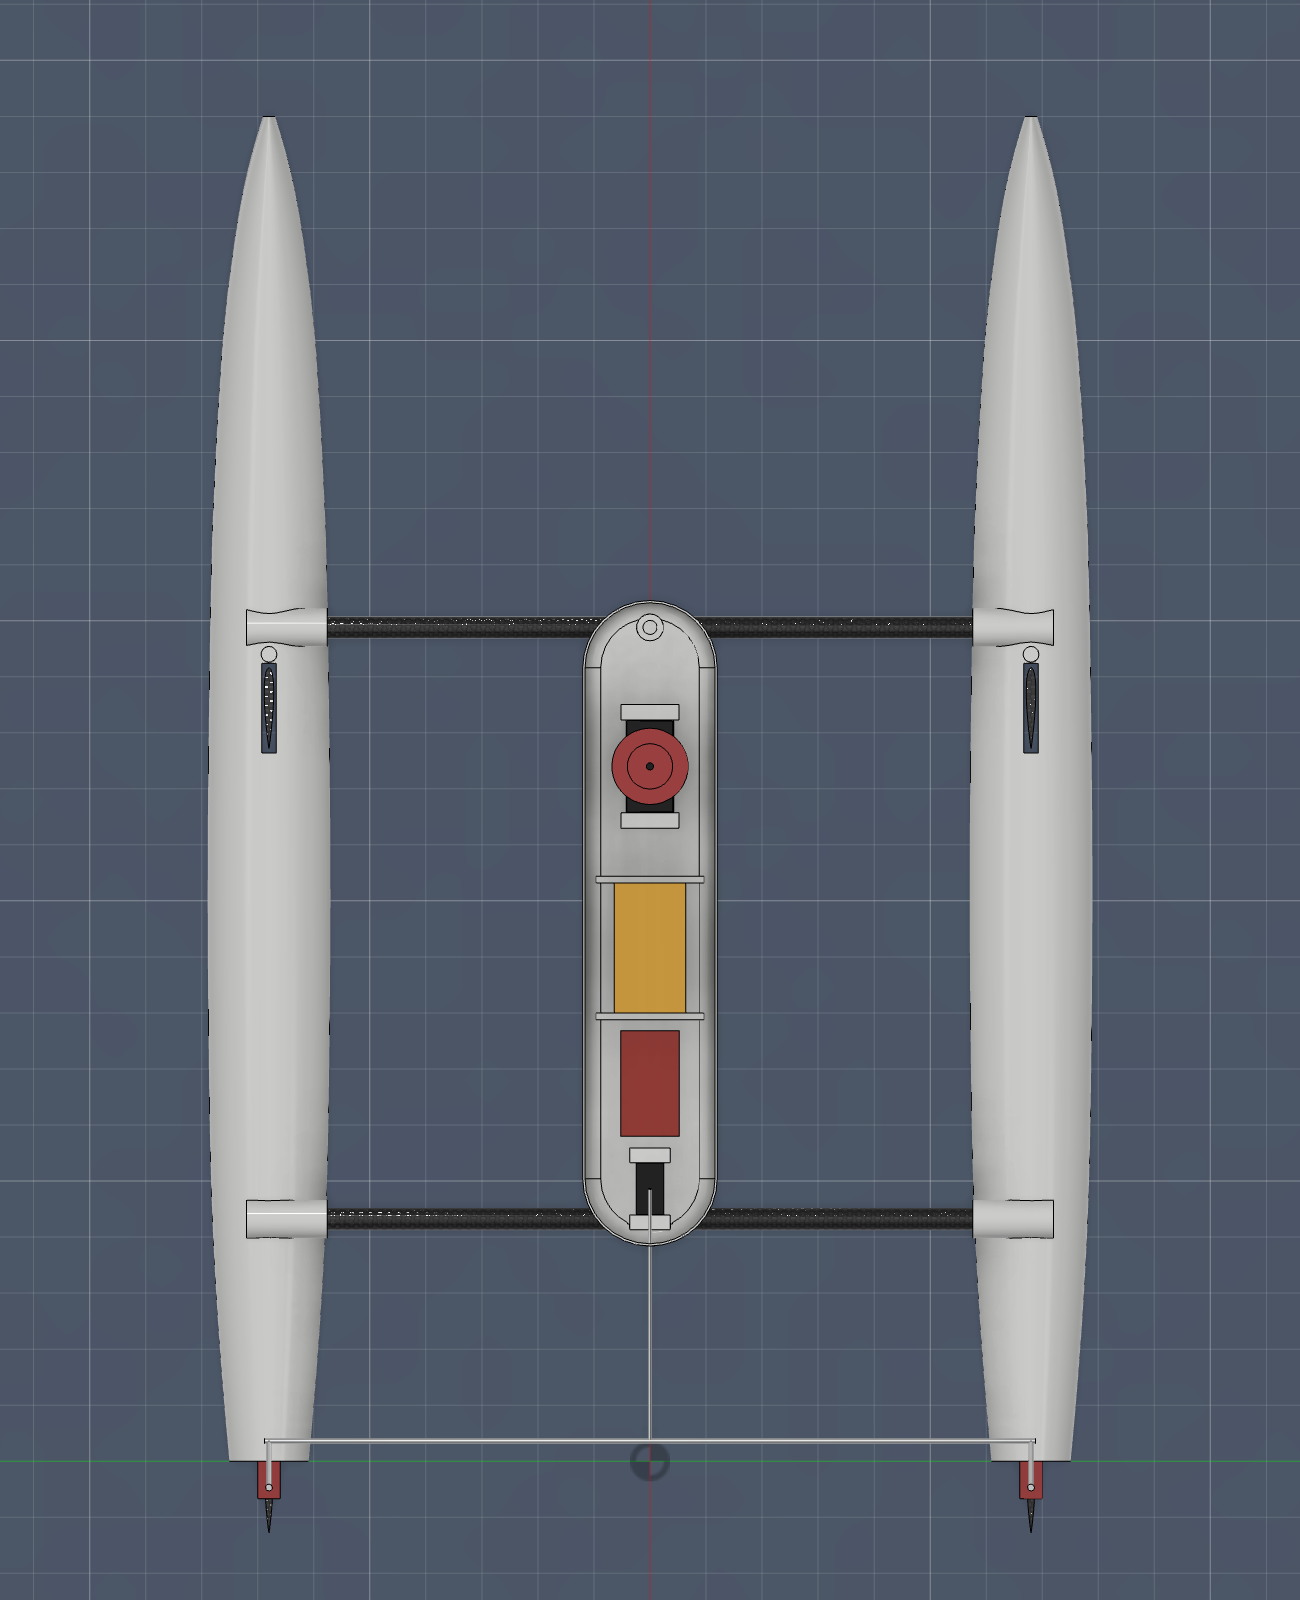
\includegraphics[width=0.55\textwidth]{../images/mini_layout_top.png}\\ \small Layout from above (lid and sails hidden): mast step, winch with stepped drum, battery, receiver, rudder servo, pushrod to the tie bar.\end{center}

\step{1. Hulls}
\begin{center}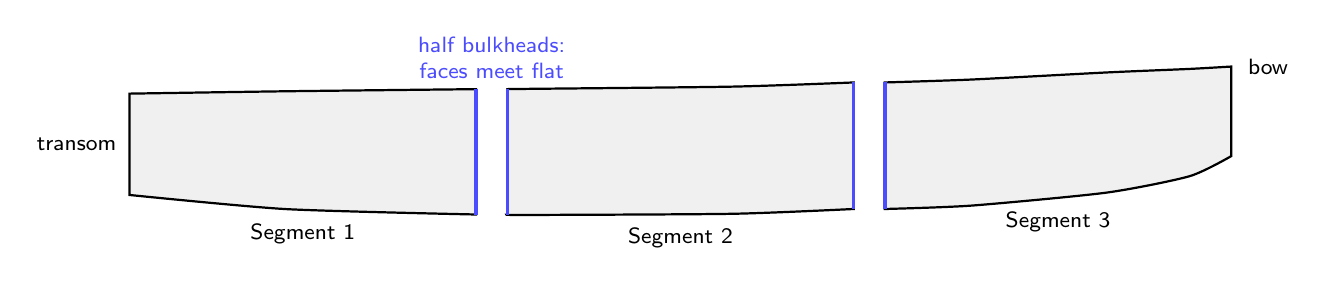
\begin{tikzpicture}\draw[thick, fill=gray!12] plot[smooth, tension=0.4] coordinates {(0.000,0.868) (1.980,0.898) (4.400,0.925)} -- plot[smooth, tension=0.4] coordinates {(4.400,-0.667) (1.980,-0.598) (0.000,-0.419)} -- cycle;
\node[font=\footnotesize] at (2.200,-0.913) {Segment 1};
\draw[thick, fill=gray!12] plot[smooth, tension=0.4] coordinates {(4.796,0.925) (5.016,0.928) (7.656,0.957) (9.196,1.010)} -- plot[smooth, tension=0.4] coordinates {(9.196,-0.597) (7.656,-0.658) (5.016,-0.673) (4.796,-0.667)} -- cycle;
\node[font=\footnotesize] at (6.996,-0.970) {Segment 2};
\draw[very thick, blue!70] (4.796,-0.667) -- (4.796,0.925);
\draw[very thick, blue!70] (4.400,-0.667) -- (4.400,0.925);
\draw[thick, fill=gray!12] plot[smooth, tension=0.4] coordinates {(9.592,1.010) (10.692,1.047) (12.408,1.137) (13.464,1.182) (13.992,1.212)} -- plot[smooth, tension=0.4] coordinates {(13.992,0.075) (13.464,-0.180) (12.408,-0.389) (10.692,-0.554) (9.592,-0.597)} -- cycle;
\node[font=\footnotesize] at (11.792,-0.756) {Segment 3};
\draw[very thick, blue!70] (9.592,-0.597) -- (9.592,1.010);
\draw[very thick, blue!70] (9.196,-0.597) -- (9.196,1.010);
\node[font=\footnotesize, blue!70, align=center] at (4.598,1.324) {half bulkheads:\\ faces meet flat};
\node[font=\footnotesize, anchor=east] at (-0.044,0.220) {transom};
\node[font=\footnotesize, anchor=west] at (14.080,1.212) {bow};\end{tikzpicture}\par\captionof{figure}{Each hull prints as three sealed segments. Sand the joint faces flat, then epoxy them face to face against a straight edge.}\end{center}
\begin{enumerate}
\item Sand the joint faces of the three segments of each hull flat on sandpaper laid on a table.
\item Dry-fit: the segments must line up on the outside. Epoxy segment 1 to 2 and 2 to 3 face to face. Hold them against a straight edge (a steel rule taped to the table) while the epoxy cures.
\item Leak test: push each hull under water for 30 seconds. A stream of bubbles marks a leak: dry, then seal it with a drop of CA or epoxy. Because every segment is its own sealed compartment, a small leak floods only one segment.
\item Drill the chainplate eye: a 1.5\,mm hole fore-aft through the small boss on the deck, 360\,mm from the transom. Drill a 1.2\,mm hole into each bow tip and epoxy in a small loop of 0.047\,in music wire for the bridle.
\end{enumerate}
\chk{each finished hull weighs about 145\,g (design value including glue) and floats level.}

\step{2. Crossbeams and frame}
\begin{center}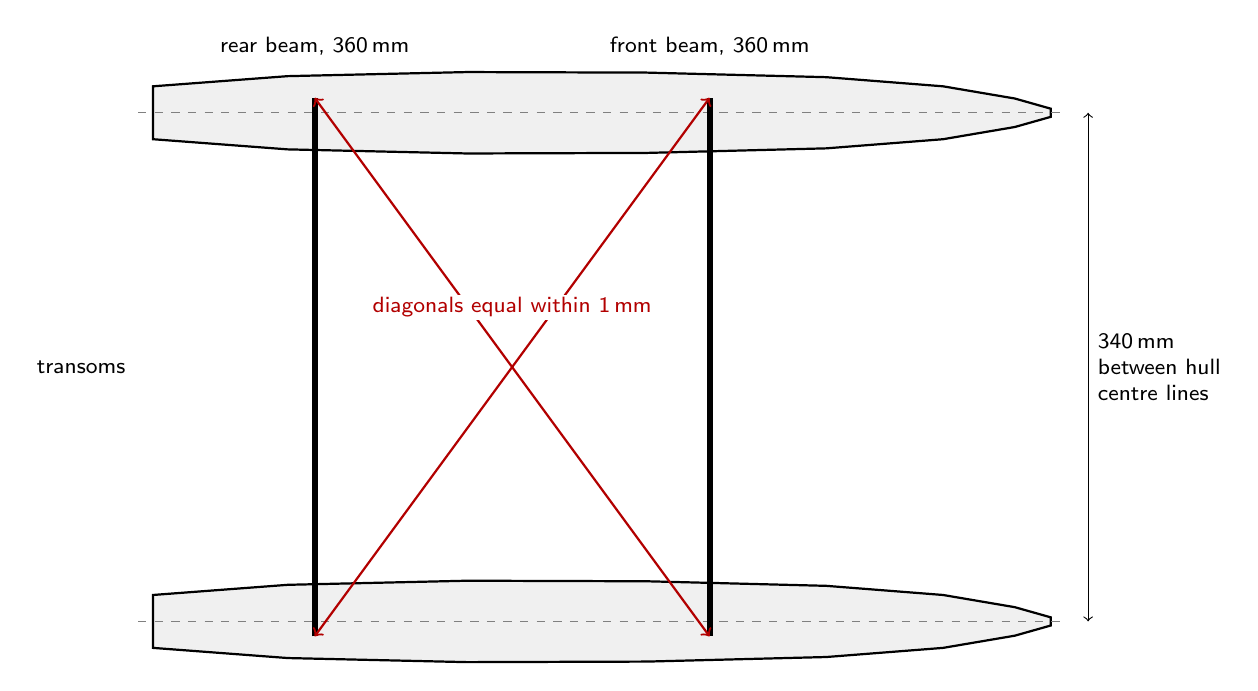
\begin{tikzpicture}\draw[thick, fill=gray!12] (0.000,3.566) -- (1.710,3.695) -- (3.990,3.747) -- (6.270,3.740) -- (8.550,3.682) -- (10.032,3.566) -- (10.944,3.411) -- (11.400,3.282) -- (11.400,3.178) -- (10.944,3.049) -- (10.032,2.894) -- (8.550,2.778) -- (6.270,2.720) -- (3.990,2.713) -- (1.710,2.765) -- (0.000,2.894) -- cycle;
\draw[dashed, gray] (-0.190,3.230) -- (11.590,3.230);
\draw[thick, fill=gray!12] (0.000,-2.894) -- (1.710,-2.765) -- (3.990,-2.713) -- (6.270,-2.720) -- (8.550,-2.778) -- (10.032,-2.894) -- (10.944,-3.049) -- (11.400,-3.178) -- (11.400,-3.282) -- (10.944,-3.411) -- (10.032,-3.566) -- (8.550,-3.682) -- (6.270,-3.740) -- (3.990,-3.747) -- (1.710,-3.695) -- (0.000,-3.566) -- cycle;
\draw[dashed, gray] (-0.190,-3.230) -- (11.590,-3.230);
\draw[line width=2.2pt] (7.068,-3.420) -- (7.068,3.420);
\draw[line width=2.2pt] (2.052,-3.420) -- (2.052,3.420);
\draw[red!70!black, thick, <->] (2.052,-3.420) -- (7.068,3.420);
\draw[red!70!black, thick, <->] (2.052,3.420) -- (7.068,-3.420);
\node[red!70!black, font=\footnotesize, fill=white, inner sep=1pt] at (4.560,0.760) {diagonals equal within 1\,mm};
\draw[<->] (11.875,-3.230) -- node[right, font=\footnotesize, align=left] {340\,mm\\between hull\\centre lines} (11.875,3.230);
\node[font=\footnotesize, above] at (7.068,3.838) {front beam, 360\,mm};
\node[font=\footnotesize, above] at (2.052,3.838) {rear beam, 360\,mm};
\node[font=\footnotesize, anchor=east] at (-0.228,0) {transoms};\end{tikzpicture}\par\captionof{figure}{Squaring the frame (top view, bows to the right). With the second hull on the beams, shift it until the two diagonals match.}\end{center}
\begin{enumerate}
\item Cut the 10\,mm carbon tube into two 360\,mm beams (score around with a knife, then snap; wear a mask when sanding carbon).
\item Epoxy both beams into the sockets of one hull. Slide the other hull on, lay the frame on a flat table and measure the two diagonals (front-left beam end to rear-right, and the reverse). Shift until they are equal within 1\,mm, then epoxy the second hull.
\end{enumerate}
\chk{hull centre lines are 340\,mm apart at both beams.}

\step{3. Rudders and steering linkage}
\begin{center}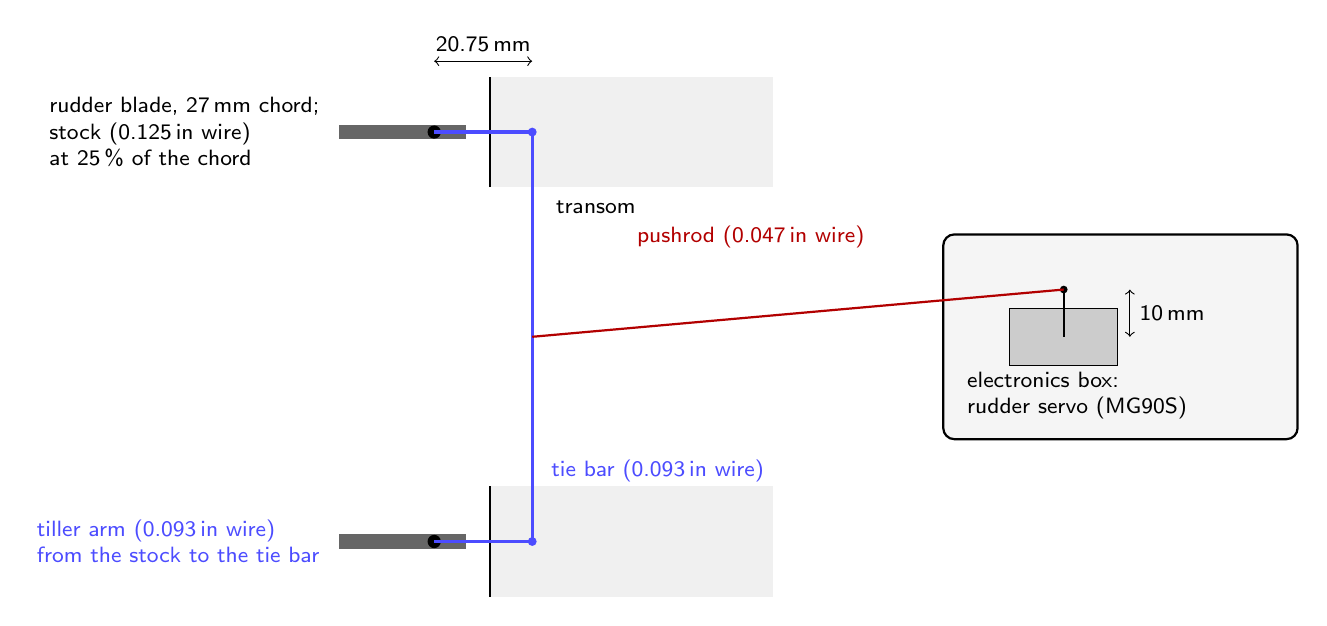
\begin{tikzpicture}\fill[gray!12] (0,1.900) rectangle (3.600,3.300);
\draw[thick] (0,1.900) -- (0,3.300);
\fill[black!60] (-1.920,2.510) rectangle (-0.300,2.690);
\fill (-0.705,2.600) circle (2.4pt);
\draw[very thick, blue!70] (-0.705,2.600) -- (0.540,2.600);
\fill[blue!70] (0.540,2.600) circle (1.6pt);
\fill[gray!12] (0,-3.300) rectangle (3.600,-1.900);
\draw[thick] (0,-3.300) -- (0,-1.900);
\fill[black!60] (-1.920,-2.690) rectangle (-0.300,-2.510);
\fill (-0.705,-2.600) circle (2.4pt);
\draw[very thick, blue!70] (-0.705,-2.600) -- (0.540,-2.600);
\fill[blue!70] (0.540,-2.600) circle (1.6pt);
\draw[very thick, blue!70] (0.540,-2.600) -- (0.540,2.600);
\draw[thick, rounded corners=4pt, fill=gray!8] (5.760,-1.3) rectangle (10.260,1.3);
\draw[fill=gray!40] (6.606,-0.360) rectangle (7.974,0.360);
\draw[thick] (7.290,0) -- (7.290,0.600);
\fill (7.290,0.600) circle (1.4pt);
\draw[thick, red!70!black] (7.290,0.600) -- (0.540,0);
\draw[<->] (-0.705,3.500) -- node[above, font=\footnotesize] {20.75\,mm} (0.540,3.500);
\draw[<->] (8.130,0) -- node[right, font=\footnotesize] {10\,mm} (8.130,0.600);
\node[font=\footnotesize, anchor=east, align=left, black] at (-2.040,2.600) {rudder blade, 27\,mm chord;\\stock (0.125\,in wire)\\at 25\,\% of the chord};
\node[font=\footnotesize, anchor=east, align=left, blue!70] at (-2.040,-2.600) {tiller arm (0.093\,in wire)\\from the stock to the tie bar};
\node[font=\footnotesize, anchor=west, align=left, blue!70] at (0.660,-1.700) {tie bar (0.093\,in wire)};
\node[font=\footnotesize, anchor=south, align=left, red!70!black] at (3.315,1.000) {pushrod (0.047\,in wire)};
\node[font=\footnotesize, anchor=west, align=left, black] at (5.940,-0.750) {electronics box:\\rudder servo (MG90S)};
\node[font=\footnotesize, anchor=west, align=left, black] at (0.720,1.650) {transom};\end{tikzpicture}\par\captionof{figure}{Steering linkage (top view, bows to the right; fore and aft to scale, the hulls drawn closer together than the real 340\,mm). Both tiller arms are the same length and the tie bar keeps the rudders parallel.}\end{center}
\begin{enumerate}
\item Drill a 3.2\,mm hole down the pivot line of each rudder blade, 6.75\,mm behind the leading edge (25\,\% of the 27\,mm chord). This balanced pivot keeps the servo load tiny.
\item Push a 0.125\,in music-wire stock through each blade and its gudgeon, epoxy the blade to the wire (not the gudgeon), and epoxy the gudgeon to the transom.
\item Bend two tiller arms from 0.093\,in wire: 20.75\,mm from the stock to the tie-bar hole. Keep the arms level, about 6\,mm above the deck, so they clear it at full rudder. Join them with a straight 0.093\,in tie bar at the transoms so the rudders stay parallel.
\item Run a 0.047\,in pushrod from the rudder servo horn (hole 10\,mm from the centre) through the slot in the rear wall of the box to the middle of the tie bar, using the Du-Bro clevis at the servo end.
\end{enumerate}
\chk{with the servo centred both rudders point straight; full servo travel gives about $\pm$20$^\circ$ of rudder.}

\step{4. Electronics box}
\begin{center}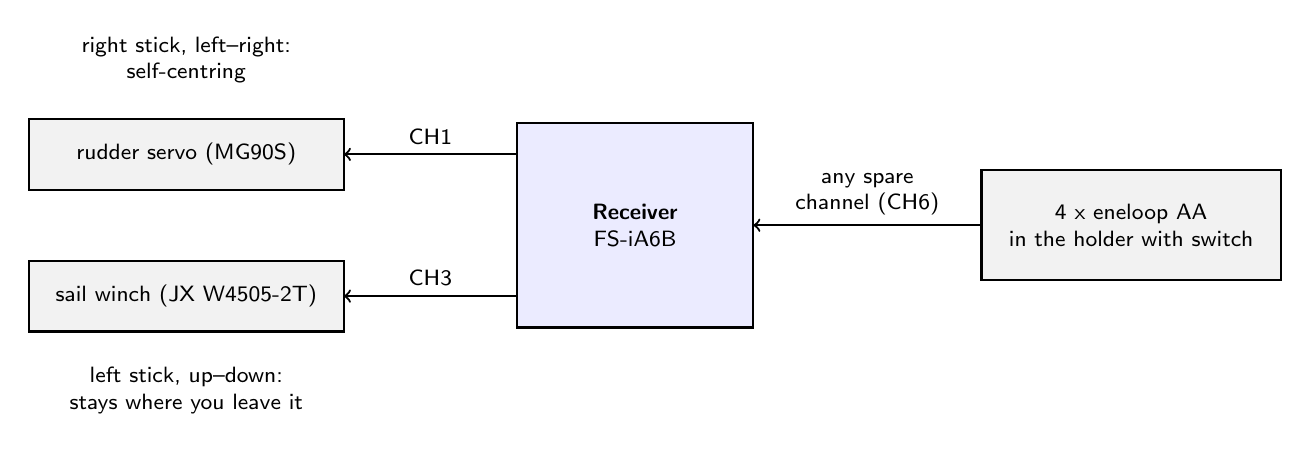
\begin{tikzpicture}\node[draw, thick, fill=blue!8, minimum width=3.0cm, minimum height=2.6cm, align=center, font=\footnotesize] at (0,0) {\textbf{Receiver}\\FS-iA6B};
\node[draw, thick, fill=gray!10, minimum width=4.0cm, minimum height=0.9cm, align=center, font=\footnotesize] at (-5.7,0.9) {rudder servo (MG90S)};
\node[draw, thick, fill=gray!10, minimum width=4.0cm, minimum height=0.9cm, align=center, font=\footnotesize] at (-5.7,-0.9) {sail winch (JX W4505-2T)};
\node[draw, thick, fill=gray!10, minimum width=3.8cm, minimum height=1.4cm, align=center, font=\footnotesize] at (6.3,0) {4 x eneloop AA\\in the holder with switch};
\draw[thick, ->] (-1.5,0.9) -- node[above, font=\footnotesize] {CH1} (-3.7,0.9);
\draw[thick, ->] (-1.5,-0.9) -- node[above, font=\footnotesize] {CH3} (-3.7,-0.9);
\draw[thick, ->] (4.4,0) -- node[above, font=\footnotesize, align=center] {any spare\\channel (CH6)} (1.5,0);
\node[font=\footnotesize, align=center] at (-5.7,2.1) {right stick, left--right:\\self-centring};
\node[font=\footnotesize, align=center] at (-5.7,-2.1) {left stick, up--down:\\stays where you leave it};\end{tikzpicture}\par\captionof{figure}{Receiver wiring. The battery powers the receiver through any free channel; both servos then take their power from the receiver.}\end{center}
\begin{enumerate}
\item Epoxy the two box halves together, and separately the two lid halves.
\item Lower the sail winch into the well between the front rails (output shaft up) until its mounting ears rest on the rails, and set the MG90S between the rear rails the same way. Lead each servo wire out sideways through the notch at the foot of a rail. Drill 1.5\,mm pilot holes through the ear holes and fix both servos with the screws supplied with them.
\chk{each case hangs from its ears, clear of the floor. The rails are drawn from the Feetech FS5115M drawing because JX does not publish the winch's ear height: if the winch case touches the bottom of the well before its ears reach the rails, put a shim (a scrap of 1\,mm plastic) under each ear.}
\item Put four charged eneloop AA cells in the Traxxas holder and set it in the battery cradle; stick the receiver on the floor between the rudder servo and the battery with double-sided tape.
\item Plug in: rudder servo to \textbf{CH1} (right stick, self-centring); sail winch to \textbf{CH3} (left stick, which stays where you leave it); battery lead to a spare channel (for example CH6). Keep both receiver antennas straight and near the top of the box.
\item Glue the printed stepped drum to the winch's round horn and screw it on.
\item Snap the box onto the two beams (the saddles clip over the 10\,mm tubes). Seal the lid seam with electrical tape before sailing.
\end{enumerate}

\step{5. Mast and standing rigging}
\begin{center}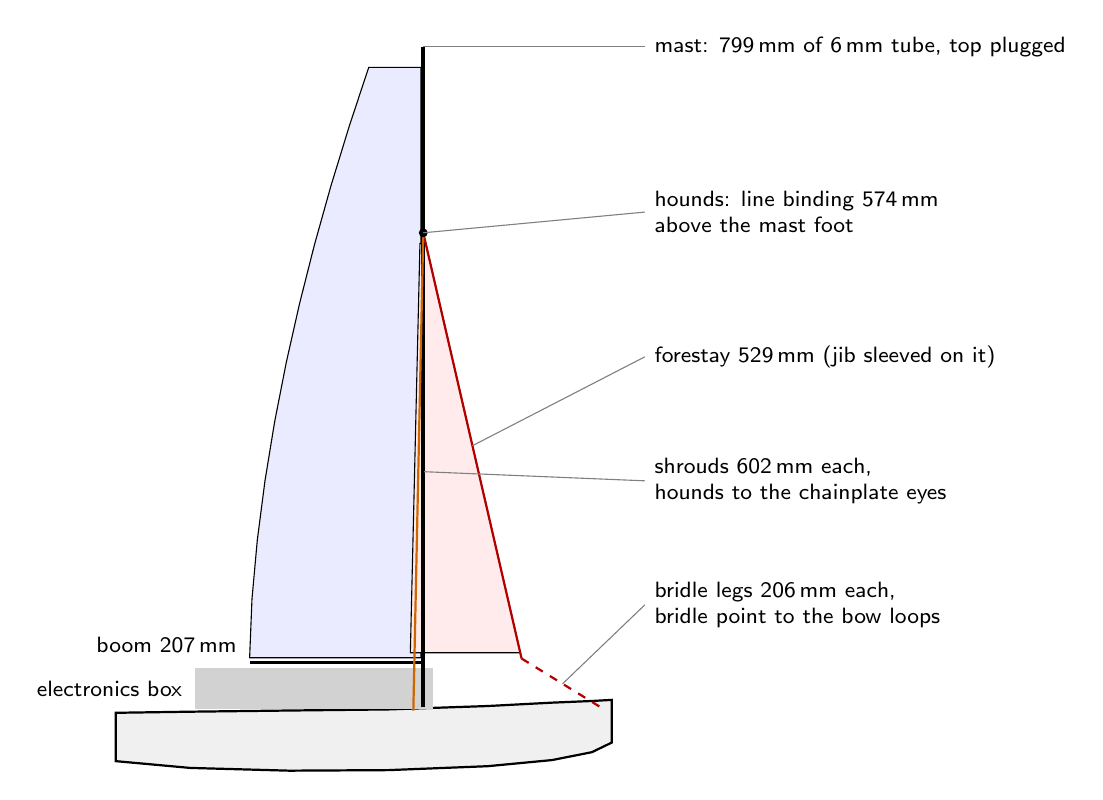
\begin{tikzpicture}\draw[thick, fill=gray!12] (0.000,0.414) -- (0.945,0.428) -- (2.205,0.443) -- (3.465,0.457) -- (4.725,0.500) -- (5.544,0.543) -- (6.048,0.564) -- (6.300,0.578) -- (6.300,0.036) -- (6.048,-0.086) -- (5.544,-0.186) -- (4.725,-0.264) -- (3.465,-0.314) -- (2.205,-0.321) -- (0.945,-0.286) -- (0.000,-0.200) -- cycle;
\fill[gray!35] (1.008,0.462) rectangle (4.032,0.987);
\draw[fill=blue!8] (3.875,1.113) -- (1.701,1.113) -- (1.731,1.863) -- (1.799,2.612) -- (1.896,3.362) -- (2.019,4.112) -- (2.166,4.862) -- (2.335,5.611) -- (2.525,6.361) -- (2.735,7.111) -- (2.965,7.860) -- (3.213,8.610) -- (3.875,8.610) -- cycle;
\draw[fill=red!8] (5.139,1.176) -- (3.742,1.176) -- (3.864,6.374) -- (3.938,6.374) -- cycle;
\draw[line width=1.6pt] (3.906,0.485) -- (3.906,8.873);
\draw[line width=1.2pt] (3.875,1.050) -- (1.701,1.050);
\draw[red!70!black, thick] (5.155,1.103) -- (3.906,6.510);
\draw[red!70!black, thick, dashed] (5.155,1.103) -- (6.195,0.462);
\draw[orange!80!black, thick] (3.906,6.510) -- (3.780,0.441);
\fill (3.906,6.510) circle (1.6pt);
\draw[gray] (6.720,8.873) -- (3.906,8.873);\node[anchor=west, font=\footnotesize, align=left] at (6.720,8.873) {mast: 799\,mm of 6\,mm tube, top plugged};
\draw[gray] (6.720,6.773) -- (3.906,6.510);\node[anchor=west, font=\footnotesize, align=left] at (6.720,6.773) {hounds: line binding 574\,mm\\above the mast foot};
\draw[gray] (6.720,4.935) -- (4.531,3.806);\node[anchor=west, font=\footnotesize, align=left] at (6.720,4.935) {forestay 529\,mm (jib sleeved on it)};
\draw[gray] (6.720,3.360) -- (3.917,3.476);\node[anchor=west, font=\footnotesize, align=left] at (6.720,3.360) {shrouds 602\,mm each,\\hounds to the chainplate eyes};
\draw[gray] (6.720,1.785) -- (5.675,0.782);\node[anchor=west, font=\footnotesize, align=left] at (6.720,1.785) {bridle legs 206\,mm each,\\bridle point to the bow loops};
\node[anchor=south east, font=\footnotesize] at (1.659,1.050) {boom 207\,mm};
\node[anchor=east, font=\footnotesize] at (0.966,0.725) {electronics box};\end{tikzpicture}\par\captionof{figure}{Rig from the side (bow to the right): stay lengths between the knots. The shrouds run down to both sides; only the near one is drawn.}\end{center}
\begin{enumerate}
\item Cut the 6\,mm tube to 799\,mm. Plug the top with epoxy. Mark the hounds (where the stays attach) 574\,mm above the mast foot and whip a tight binding of line there, glued with CA.
\item Stand the mast in the socket on the box floor through the lid hole.
\item Tie the stays from braided line (lengths between knots): forestay 529\,mm from the hounds to the bridle point; two bridle legs of 206\,mm from the bridle point to the bow loops; two shrouds of 602\,mm from the hounds to the chainplate eyes.
\item Cut the 4\,mm tube to a 207\,mm boom. Tie a loose loop of line through its front end around the mast so the boom sits about 5\,mm above the lid and swings freely.
\end{enumerate}
\chk{the mast stands straight from the side and from behind; all stays are just tight.}

\step{6. Sails}
\begin{center}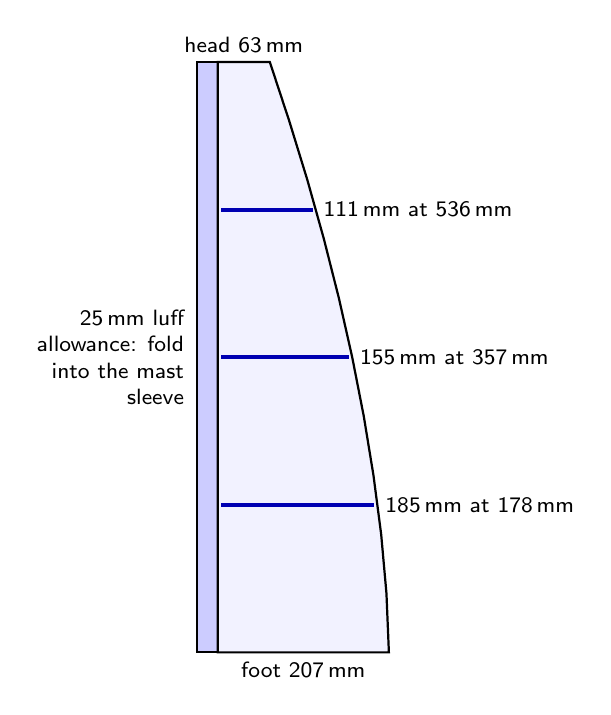
\begin{tikzpicture}\fill[blue!20] (-0.263,0) rectangle (0,7.497);
\draw[thick, fill=blue!5] (0,0) -- (2.174,0.000) -- (2.143,0.750) -- (2.076,1.499) -- (1.978,2.249) -- (1.855,2.999) -- (1.708,3.749) -- (1.539,4.498) -- (1.349,5.248) -- (1.139,5.998) -- (0.909,6.747) -- (0.662,7.497) -- (0,7.497) -- cycle;
\draw[thick] (-0.263,0) rectangle (0,7.497);
\node[font=\footnotesize, anchor=east, align=right] at (-0.304,3.749) {25\,mm luff\\allowance: fold\\into the mast\\sleeve};
\draw[line width=1.4pt, blue!70!black] (0.042,1.874) -- (1.989,1.874) node[right, font=\footnotesize, black] {185\,mm at 178\,mm};
\draw[line width=1.4pt, blue!70!black] (0.042,3.749) -- (1.666,3.749) node[right, font=\footnotesize, black] {155\,mm at 357\,mm};
\draw[line width=1.4pt, blue!70!black] (0.042,5.623) -- (1.204,5.623) node[right, font=\footnotesize, black] {111\,mm at 536\,mm};
\node[font=\footnotesize, below] at (1.087,0) {foot 207\,mm};
\node[font=\footnotesize, above] at (0.331,7.497) {head 63\,mm};\end{tikzpicture}\par\captionof{figure}{Mainsail laid flat: batten lengths and their heights above the foot. The 1:1 pattern has the full outline.}\end{center}
\begin{enumerate}
\item Print \texttt{mini/manual/sail\_patterns\_1to1.pdf} at 100\,\% (large-format print, or tile it). The 100\,mm scale bar must measure 100\,mm.
\item Lay the Icarex on the pattern and cut the main and jib with a hot knife or scissors. The main needs the extra 25\,mm on the luff for the mast sleeve.
\item Main: fold the 25\,mm sleeve and close it with sail tape so it slides over the mast. Cut three battens from 1.2\,mm carbon rod (185, 155, 111\,mm) and tape them on at 178, 357, 536\,mm above the foot.
\item Jib: fold a 10\,mm sleeve along the 508\,mm luff around the forestay line.
\item Reinforce the head, tack and clew of both sails with two layers of sail tape and melt a 2\,mm hole in each clew.
\end{enumerate}

\step{7. Sheets and drum}
Both sheets end on the one drum, so one stick moves both sails.
\begin{center}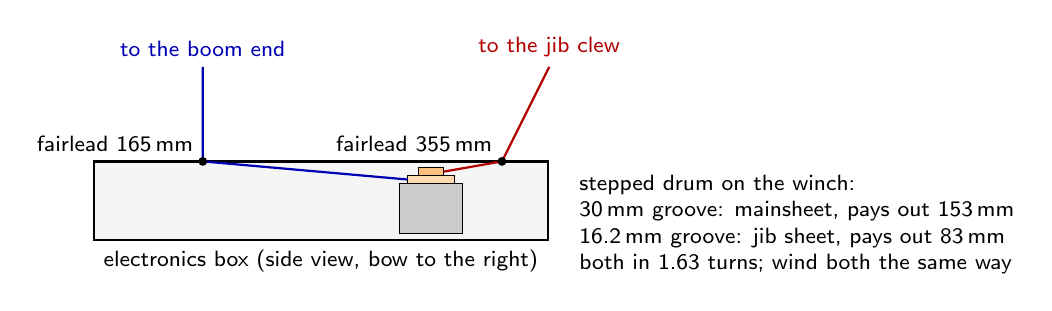
\begin{tikzpicture}\draw[thick, fill=gray!8] (1.920,0.880) rectangle (7.680,1.880);
\node[font=\footnotesize, anchor=north] at (4.800,0.880) {electronics box (side view, bow to the right)};
\draw[fill=gray!40] (5.800,0.960) rectangle (6.600,1.600);
\draw[fill=orange!30] (5.900,1.600) rectangle (6.500,1.700);
\draw[fill=orange!50] (6.038,1.700) rectangle (6.362,1.800);
\draw[blue!70!black, thick] (5.900,1.650) -- (3.300,1.880) -- (3.300,3.080) node[above, font=\footnotesize, align=center] {to the boom end};
\draw[red!70!black, thick] (6.362,1.750) -- (7.100,1.880) -- (7.700,3.080) node[above, font=\footnotesize, align=center] {to the jib clew};
\fill (3.300,1.880) circle (1.6pt) node[above left, font=\footnotesize] {fairlead 165\,mm};
\fill (7.100,1.880) circle (1.6pt) node[above left, font=\footnotesize] {fairlead 355\,mm};
\node[font=\footnotesize, align=left, anchor=west] at (7.960,1.080) {stepped drum on the winch:\\30\,mm groove: mainsheet, pays out 153\,mm\\16.2\,mm groove: jib sheet, pays out 83\,mm\\both in 1.63 turns; wind both the same way};\end{tikzpicture}\par\captionof{figure}{Both sheets on the one drum. Fairlead distances are measured from the transoms.}\end{center}
\begin{itemize}
\item Mainsheet: from the boom end, down through the lid fairlead 165\,mm from the transom, to the \textbf{30\,mm groove}.
\item Jib sheet: from the jib clew, down through the fairlead 355\,mm from the transom, to the \textbf{16.2\,mm groove}.
\item Wind both sheets the same way. From sheeted in to fully eased the mainsheet pays out 153\,mm and the jib sheet 83\,mm. Both take 1.63 drum turns, which is why the grooves have different diameters.
\end{itemize}

\step{8. Radio setup}
\begin{enumerate}
\item Bind the receiver to the transmitter (follow the FlySky manual) and select an airplane model.
\item Set the CH3 end points so full stick travel turns the drum 1.63 turns. If the winch makes 2 turns at 100\,\%, that is about 82\,\%. Reverse CH3 if needed so that stick down means sheets in.
\item Set CH1 so the right stick steers the boat the way you expect: stick right, bow turns right.
\item Use the radio's failsafe function: on signal loss, rudders centred and sheets eased. An eased cat stops and drifts instead of sailing away.
\end{enumerate}

\step{9. Balance and float test}
\begin{enumerate}
\item Rig the boat. Balance it on two fingers under the beams: it should balance about 258\,mm forward of the transoms. If not, move the battery.
\item Float it in a tub: the hulls should sit level, about 24\,mm deep. Leave it 10 minutes and check for water in the box.
\end{enumerate}

\step{10. First sail}
\begin{itemize}
\item Pick 3 to 8\,kn of wind, a small pond, and a way to retrieve the boat that does not involve swimming (a friend's kayak, or a long pole and line). A capsized catamaran does not right itself.
\item Start on a beam reach with the sheets half out. Sheet in until the boat accelerates; ease when a hull starts to lift.
\item Above about 8\,kn, ease the sheets to keep the windward hull down.
\item Watch the bows. A catamaran more often trips over its bows (pitchpoles) than capsizes sideways. The analysis puts the bow-burying limit at about 7.5 / 8.5 / 10 / 13.5\,kn of wind at 60 / 90 / 120 / 150$^\circ$ off the wind. Near those winds, ease the sheets as soon as the leeward bow starts to dig.
\item If the boat keeps turning away from the wind, sheet the jib less (the jib rides 4$^\circ$ wider than the main on the drum) or move the mast step aft. If it keeps turning into the wind, do the opposite.
\end{itemize}

\section{Troubleshooting}
\begin{tabularx}{\textwidth}{>{\raggedright}p{4cm}X}
\toprule
Symptom & Fix \\
\midrule
Water inside a hull segment & Leak test that segment again; seal with CA; paint the outside with thinned epoxy \\
Winch stalls or jitters & Check the battery charge; reduce the CH3 end points; make sure no line is caught under the drum \\
Rudders do not centre & Re-bend the pushrod or adjust the clevis; set CH1 sub-trim \\
Boat will not tack & Sail faster before turning; turn gradually with full rudder; ease the jib during the turn \\
Nose dives in gusts & Ease both sheets earlier; move the battery aft \\
\bottomrule
\end{tabularx}

\appendix
\section{Engineering numbers}
Hydrostatics (fresh water): mass 755\,g; waterline at z=-6.8\,mm on the design reference; hull volume 1546\,cm$^3$ per hull; maximum righting moment 1.20\,N\,m from the heeled-hull calculation (largest righting arm 162\,mm at 8$^\circ$, capsize near 80$^\circ$); largest bow-down moment the hulls can resist 0.82\,N\,m on two hulls, 0.58\,N\,m on one; heeling arm 0.42\,m.

\noindent Predicted boat speed in m/s (* = sails eased to keep the windward hull down):
\begin{center}
\begin{tabular}{cccc}
\toprule
True wind (kn) & TWA 60$^\circ$ & TWA 90$^\circ$ & TWA 105$^\circ$ \\
\midrule
2 & 0.39 & 0.43 & 0.41 \\
4 & 0.89 & 0.95 & 0.89 \\
6 & 1.39 & 1.51 & 1.41 \\
8 & 1.87* & 2.13* & 2.07 \\
10 & 2.01* & 2.13* & 2.13* \\
12 & 2.11* & 2.13* & 2.13* \\
14 & 2.11* & 2.13* & 2.13* \\
\bottomrule
\end{tabular}
\end{center}
These come from the same velocity-prediction code as the 1\,m boat. Hull friction uses the ITTC-57 line; wave drag uses the Michell thin-ship integral with catamaran interference; sail forces use a lift/drag model. The code and its validation checks are in \texttt{analysis/vpp.py} and \texttt{mini/mini\_analysis.py}. They are predictions until measured with GPS on the water.

\section{Parts cost of the 1\,m build-first boat}
{\small
\begin{longtable}{p{1.5cm}p{4.3cm}p{5.0cm}cp{1.2cm}p{1.2cm}}
\toprule
\textbf{Group} & \textbf{Item} & \textbf{Used for} & \textbf{Qty} & \textbf{Unit} & \textbf{Total} \\
\midrule\endhead
Radio & FlySky FS-i6X + FS-iA6B receiver & 4 channels used: rudder, traveler, jib, mainsheet & 1 & \$69.99 & \$69.99 \\
Radio & AA alkaline x4 & transmitter power & 1 & \$2.99 & \$2.99 \\
Servos & JX W4505-4T sail winch servo & traveler (about 209 mm of car travel, rig model) & 1 & \$11.13 & \$11.13 \\
Servos & JX W4505-2T sail winch servo & jib sheet (about 82 mm of sheet, rig model) & 1 & \$11.13 & \$11.13 \\
Servos & Feetech FS5115M standard servo & mainsheet tension & 1 & \$32.06 & \$32.06 \\
Servos & MG90S metal-gear micro servo & rudders via pushrod + tie bar & 1 & \$2.59 & \$2.59 \\
Power & Panasonic eneloop AA 2000 mAh, 4-pack & receiver pack (4.8 V) & 1 & \$17.99 & \$17.99 \\
Power & Traxxas 4-cell AA holder with switch (TRA1523) & receiver battery box + on/off & 1 & \$4.00 & \$4.00 \\
Printed & PETG filament 1 kg & hulls, pod, lid, rudder-servo bracket and cover, rudders, boards, gudgeons, tracks, cars, mast fairing and fittings (~1.5 kg used, 1 m manual print list) & 2 & \$13.99 & \$27.98 \\
Carbon & Carbon tube 16 x 14 mm x 1 m & two 600 mm crossbeams & 2 & \$27.46 & \$54.92 \\
Carbon & Carbon tube 12 x 10 mm x 1 m & two-piece mast (1.3 m) & 2 & \$12.26 & \$24.52 \\
Carbon & Carbon tube 10 x 8 mm x 1 m & mast joiner spigot (150 mm) and pod beam (600 mm) & 1 & \$16.15 & \$16.15 \\
Carbon & Carbon tube 8 x 7 mm x 1 m & boom (345 mm) & 1 & \$17.20 & \$17.20 \\
Carbon & Carbon rod 1.2 mm x 2 m & 8 battens (2.01 m in all; finish them from the 1 m rod) & 1 & \$5.25 & \$5.25 \\
Carbon & Carbon rod 1.2 mm x 1 m & the last batten, daggerboard joint rods (4 x 80 mm) & 1 & \$3.47 & \$3.47 \\
Hardware & Music wire 0.156 in & rudder stocks, tie bar & 2 & \$4.99 & \$9.98 \\
Hardware & Music wire 0.093 in & rudder pushrod, track end-stop turning pins, gooseneck pin, boom sheet eye & 1 & \$3.99 & \$3.99 \\
Hardware & Du-Bro micro pushrod system & clevises & 1 & \$8.55 & \$8.55 \\
Sails & Icarex PC31 ripstop polyester, 1 m & main + jib (0.40 m2) & 1 & \$21.99 & \$21.99 \\
Sails & Ripstop sail tape 2 in, half roll & luff, batten pockets, corners & 1 & \$9.65 & \$9.65 \\
Rigging & Braided PE line 30 lb & stays, bridle, sheets & 1 & \$14.43 & \$14.43 \\
Adhesives & BSI 30-minute epoxy 9 oz & hull joints, beams, fittings & 1 & \$22.99 & \$22.99 \\
Adhesives & BSI gap-filling CA 1/2 oz & small parts & 1 & \$4.79 & \$4.79 \\
\midrule
& \textbf{Total} & & & & \textbf{\$397.74} \\
\bottomrule
\end{longtable}}
If you build the mini first, the radio and the NiMH pack carry over, which lowers the 1\,m boat's extra cost by \$94.97.

\section{Parts cost of the v2.3 foiling kit}
The kit is sized for the v2.3 foils in the CAD model: NACA\,4412 wings 180\,x\,50\,mm at $+1.5^\circ$, NACA\,0012 elevators 160\,x\,28\,mm at $-0.5^\circ$ (nose down), and 60\,mm-chord struts. The foiling rudders end 18\,mm lower than the build-first ones, in a printed trim pod: bond a 8\,mm extension (\url{stl/Foiling_Rudder_Extension_x2.stl}) and then the pod (\url{stl/Elevator_Trim_Pod_x2.stl}, 45\,x\,9\,x\,14\,mm) under each blade. The elevator passes through the pod's slot, pivots on a 2\,mm carbon pin at its quarter chord, and is clamped by two M2 set screws 12\,mm behind the pin (one from above, one from below): one turn moves it about $1.9^\circ$, so it can be trimmed on the water. Printable cores with 0.5\,mm recesses for the carbon caps are in \url{stl/} (\texttt{Foil\_Core\_*}, \texttt{Foil\_Flap\_x2}). The foils are printed PETG cores with unidirectional carbon caps (4 layers per face), laminated with epoxy; the caps take about 5.0\,m of the 7.3\,m of tape listed. The kit also includes flap hinges, the ride-height wands and their linkage. It is added to the 1\,m boat after the build-first version sails.
{\small
\begin{longtable}{p{1.5cm}p{4.3cm}p{5.0cm}cp{1.2cm}p{1.2cm}}
\toprule
\textbf{Group} & \textbf{Item} & \textbf{Used for} & \textbf{Qty} & \textbf{Unit} & \textbf{Total} \\
\midrule\endhead
Printed & PETG filament 1 kg & L-foil, elevator and flap cores, trim pods, ride-height linkage (~290 g, 1 m manual print list) & 1 & \$13.99 & \$13.99 \\
Carbon & Unidirectional carbon tape 2 in x 12 ft & spar caps: 4 layers per face on struts, wings, elevators & 2 & \$19.95 & \$39.90 \\
Adhesives & EL2 laminating epoxy 500 g & wet-out of the caps & 1 & \$20.70 & \$20.70 \\
Carbon & Carbon rod 1.2 mm x 1 m & flap hinge pins & 1 & \$3.47 & \$3.47 \\
Carbon & Carbon rod 2 mm x 1 m & two 300 mm ride-height wands, elevator pivot pins, wand and bellcrank axles, L-foil core dowels & 1 & \$8.85 & \$8.85 \\
Hardware & Music wire 0.047 in & wand-to-flap pushrods & 1 & \$3.99 & \$3.99 \\
Hardware & Du-Bro micro pushrod system & clevises for the flap linkage & 1 & \$8.55 & \$8.55 \\
Hardware & M2 x 6 mm stainless set screw, cup point (Bolt Depot 8697) & elevator trim screws, two per trim pod & 4 & \$0.43 & \$1.72 \\
\midrule
& \textbf{Total} & & & & \textbf{\$101.17} \\
\bottomrule
\end{longtable}}

\section{Price sources (read 23-24 September 2026)}
{\small
\begin{itemize}
\item HobbyTown: \url{https://www.hobbytown.com/flysky-i6x-6channel-afhds-2a-air-radio-system-w-ia6b-receiver-fsy-i6xia6b/p1674181}
\item HobbyTown (EcoPower AA x4 add-on): \url{https://www.hobbytown.com/flysky-fsgt2e-2channel-transmitter-w-fsa3-receiver-fsy-fs-gt2ea3/p1592822}
\item AliExpress: listed \$5.79 at 48\% off; full price used (2026-09-23; on 2026-10-04 the page showed a bot check, not re-checked): \url{https://www.aliexpress.com/item/1005003265131874.html}
\item Waveshare: \url{https://www.waveshare.com/mg90s-servo.htm}
\item Walmart, sold by My Battery Supplier (BK-3MCCA4BA, in stock 2026-10-04): \url{https://www.walmart.com/ip/Panasonic-Eneloop-BK-3MCCA4BA-Pre-Charged-Nickel-Metal-Hydride-AA-Rechargeable-Batteries-4-Battery-Pack/39111776}
\item HobbyTown: \url{https://www.hobbytown.com/traxxas-4cell-aa-battery-holder-w-switch-cover-tra1523/p49945}
\item Elegoo US: \url{https://us.elegoo.com/products/rapid-petg-filament-1-75mm-colored-1kg}
\item CST CS-525 1M: \url{https://www.cstsales.com/Carbon_Fiber_Tubes.html}
\item CST CS-316 1M: \url{https://www.cstsales.com/carbon_rods.html}
\item K\&S 0.125 in x 12 in: \url{https://ksmetals.com/collections/12-long-music-wire}
\item HobbyTown: \url{https://www.hobbytown.com/dubro-pushrod-system-micro-dub847/p29360}
\item Jones Airfoils, per metre (138 cm wide); 1 m price read 2026-09-23 (on 2026-10-04 the page showed local currency; 5 m or more is \$18.49/m): \url{https://jonesairfoils.com/products/icarex}
\item kiteboarding.com: 10 ft cut, \$15.00 roll less \$8.50 (2026-10-04): \url{https://kiteboarding.com/proddetail.asp?prod=ripstop_2inch}
\item Walmart, PowerPro 30 lb x 150 yd (read 2026-09-24; the original eBay listing had ended): \url{https://www.walmart.com/ip/PowerPro-Braided-Fishing-Line-30lb-x-150yd-ylw-21100300150Y/17117880}
\item HobbyTown BSI205: \url{https://www.hobbytown.com/bob-smith-industries-slowcure-30-minute-epoxy-4-1-2oz-bsi205/p37085}
\item HobbyTown: \url{https://www.hobbytown.com/bob-smith-industries-instacure-gap-filling-ca-1-2oz-bsi106/p37055}
\item HobbyTown: \url{https://www.hobbytown.com/ecopower-640t-13g-waterproof-metal-gear-digital-sub-micro-servo-ecp-640t/p859667}
\item MicroBattery (out of stock on 2026-10-04): \url{https://www.microbattery.com/panasonic-bk-3mcca4ba-eneloop-aa-2100-cycle-ni-mh-pre-charged-rechargeable-batteries-4-pack80.html}
\item Wind Catcher RC (price from a search listing; the site blocked this connection on 2026-10-04): \url{https://windcatcherrc.com/product/carbon-fiber-tube-16mm-x-14mm-x-1000mm/}
\item HobbyTown: \url{https://www.hobbytown.com/bob-smith-industries-quickcure-5-minute-epoxy-4-1-2oz-bsi201/p37081}
\item HobbyTown: \url{https://www.hobbytown.com/bob-smith-industries-quickcure-5-minute-epoxy-9o-bsi202/p37082}
\item Pololu: \url{https://www.pololu.com/product/3426}
\item RMRC 16X14X1M-CF-TUBE (in stock 2026-10-04): \url{https://www.readymaderc.com/products/details/86475-carbon-fiber-tube-16mm-x-14mm-1m-long}
\item RMRC: \url{https://www.readymaderc.com/products/details/carbon-fiber-tube-12mm-x-10mm-1m-long}
\item HobbyTown BSI206: \url{https://www.hobbytown.com/bob-smith-industries-slowcure-30-minute-epoxy-9o-bsi206/p37086}
\item CST CU-379: 2 in unidirectional carbon, 0.005 in, 12 ft: \url{https://www.cstsales.com/heat_tack.html}
\item Easy Composites EL2, 500 g kit: \url{https://www.easycomposites.us/el2-epoxy-laminating-resin}
\item Bolt Depot, per piece (read 2026-09-25): \url{https://boltdepot.com/Product-Details?product=8697}
\end{itemize}}
Two prices carry extra uncertainty: the JX winch (AliExpress listed it on sale; the full price is used here) and the 16\,x\,14\,mm carbon tube (price taken from a search listing because the store's page was not reachable).
\end{document}
